\chapter{Background}
\label{chap:background}

\textit{Introduzione sugli argomenti teorici toccati nell'ambito delle Intelligenze Artificiali, sui linguaggi di programmazione e le tecnologie utilizzate durante il tirocinio}

\section{Argomenti teorici}


\subsection{Intelligenza Artificiale}

Per intelligenza artificiale (IA), in inglese \textit{Artificial Intelligence(AI)}, si intende l'abilità di macchine e computer di comprendere ed imparare, risolvere problemi, prendere decisioni, simulare creatività e autonomia, svolgere compiti come se fossero esseri umani, individui dotati di intelligenza. \\
Proprio quest'ultimo termine, \textit{"Intelligence"}, fu utilizzato assieme ad \textit{"Artificial"} da J. McCarthy nel 1956, quando egli coniò l'espressione, definendola \textit{"the science and engineering of making intelligent machines"}. 
Ciò nonostante, tuttora si fatica ancora a fornire una definizione solida di cosa si intenda con il termine e quale sia la natura esatta del suo oggetto di studio, il che è in un certo senso uno degli aspetti più affascinanti del campo dell'IA. Questa incertezza è riconducibile all'ambiguità e la difficoltà nel fornire una risposta precisa alla domanda "Cosa si intende per "intelligenza"?", come ammette lo stesso McCarthy in una sua intervista\footcite{article:what-is-ai}. Il fulcro del problema sta nella difficoltà a fornire una spiegazione al termine senza ricadere su un'associazione all'intelligenza umana e se la capacità dei computer di svolgere certi compiti e risolvere alcuni problemi possa essere prova che siano dotate di essa. \\

Nonostante queste difficoltà concettuali, l'IA ha trovato applicazioni concrete, ha dimostrato la sua utilità in diversi campi e si è estesa lungo diverse aree di ricerca anche molto diverse tra loro.
La sotto-area più rilevante per questa tesi è quella del \textit{Machine Learning},
che si è sviluppata a partire dagli anni '80 in una serie di concetti dedicati 
e ambiti di applicazione come mostrato in Figura \ref{fig:diagram-ai-sub-concepts}.

\begin{figure}[H]
    \centering
    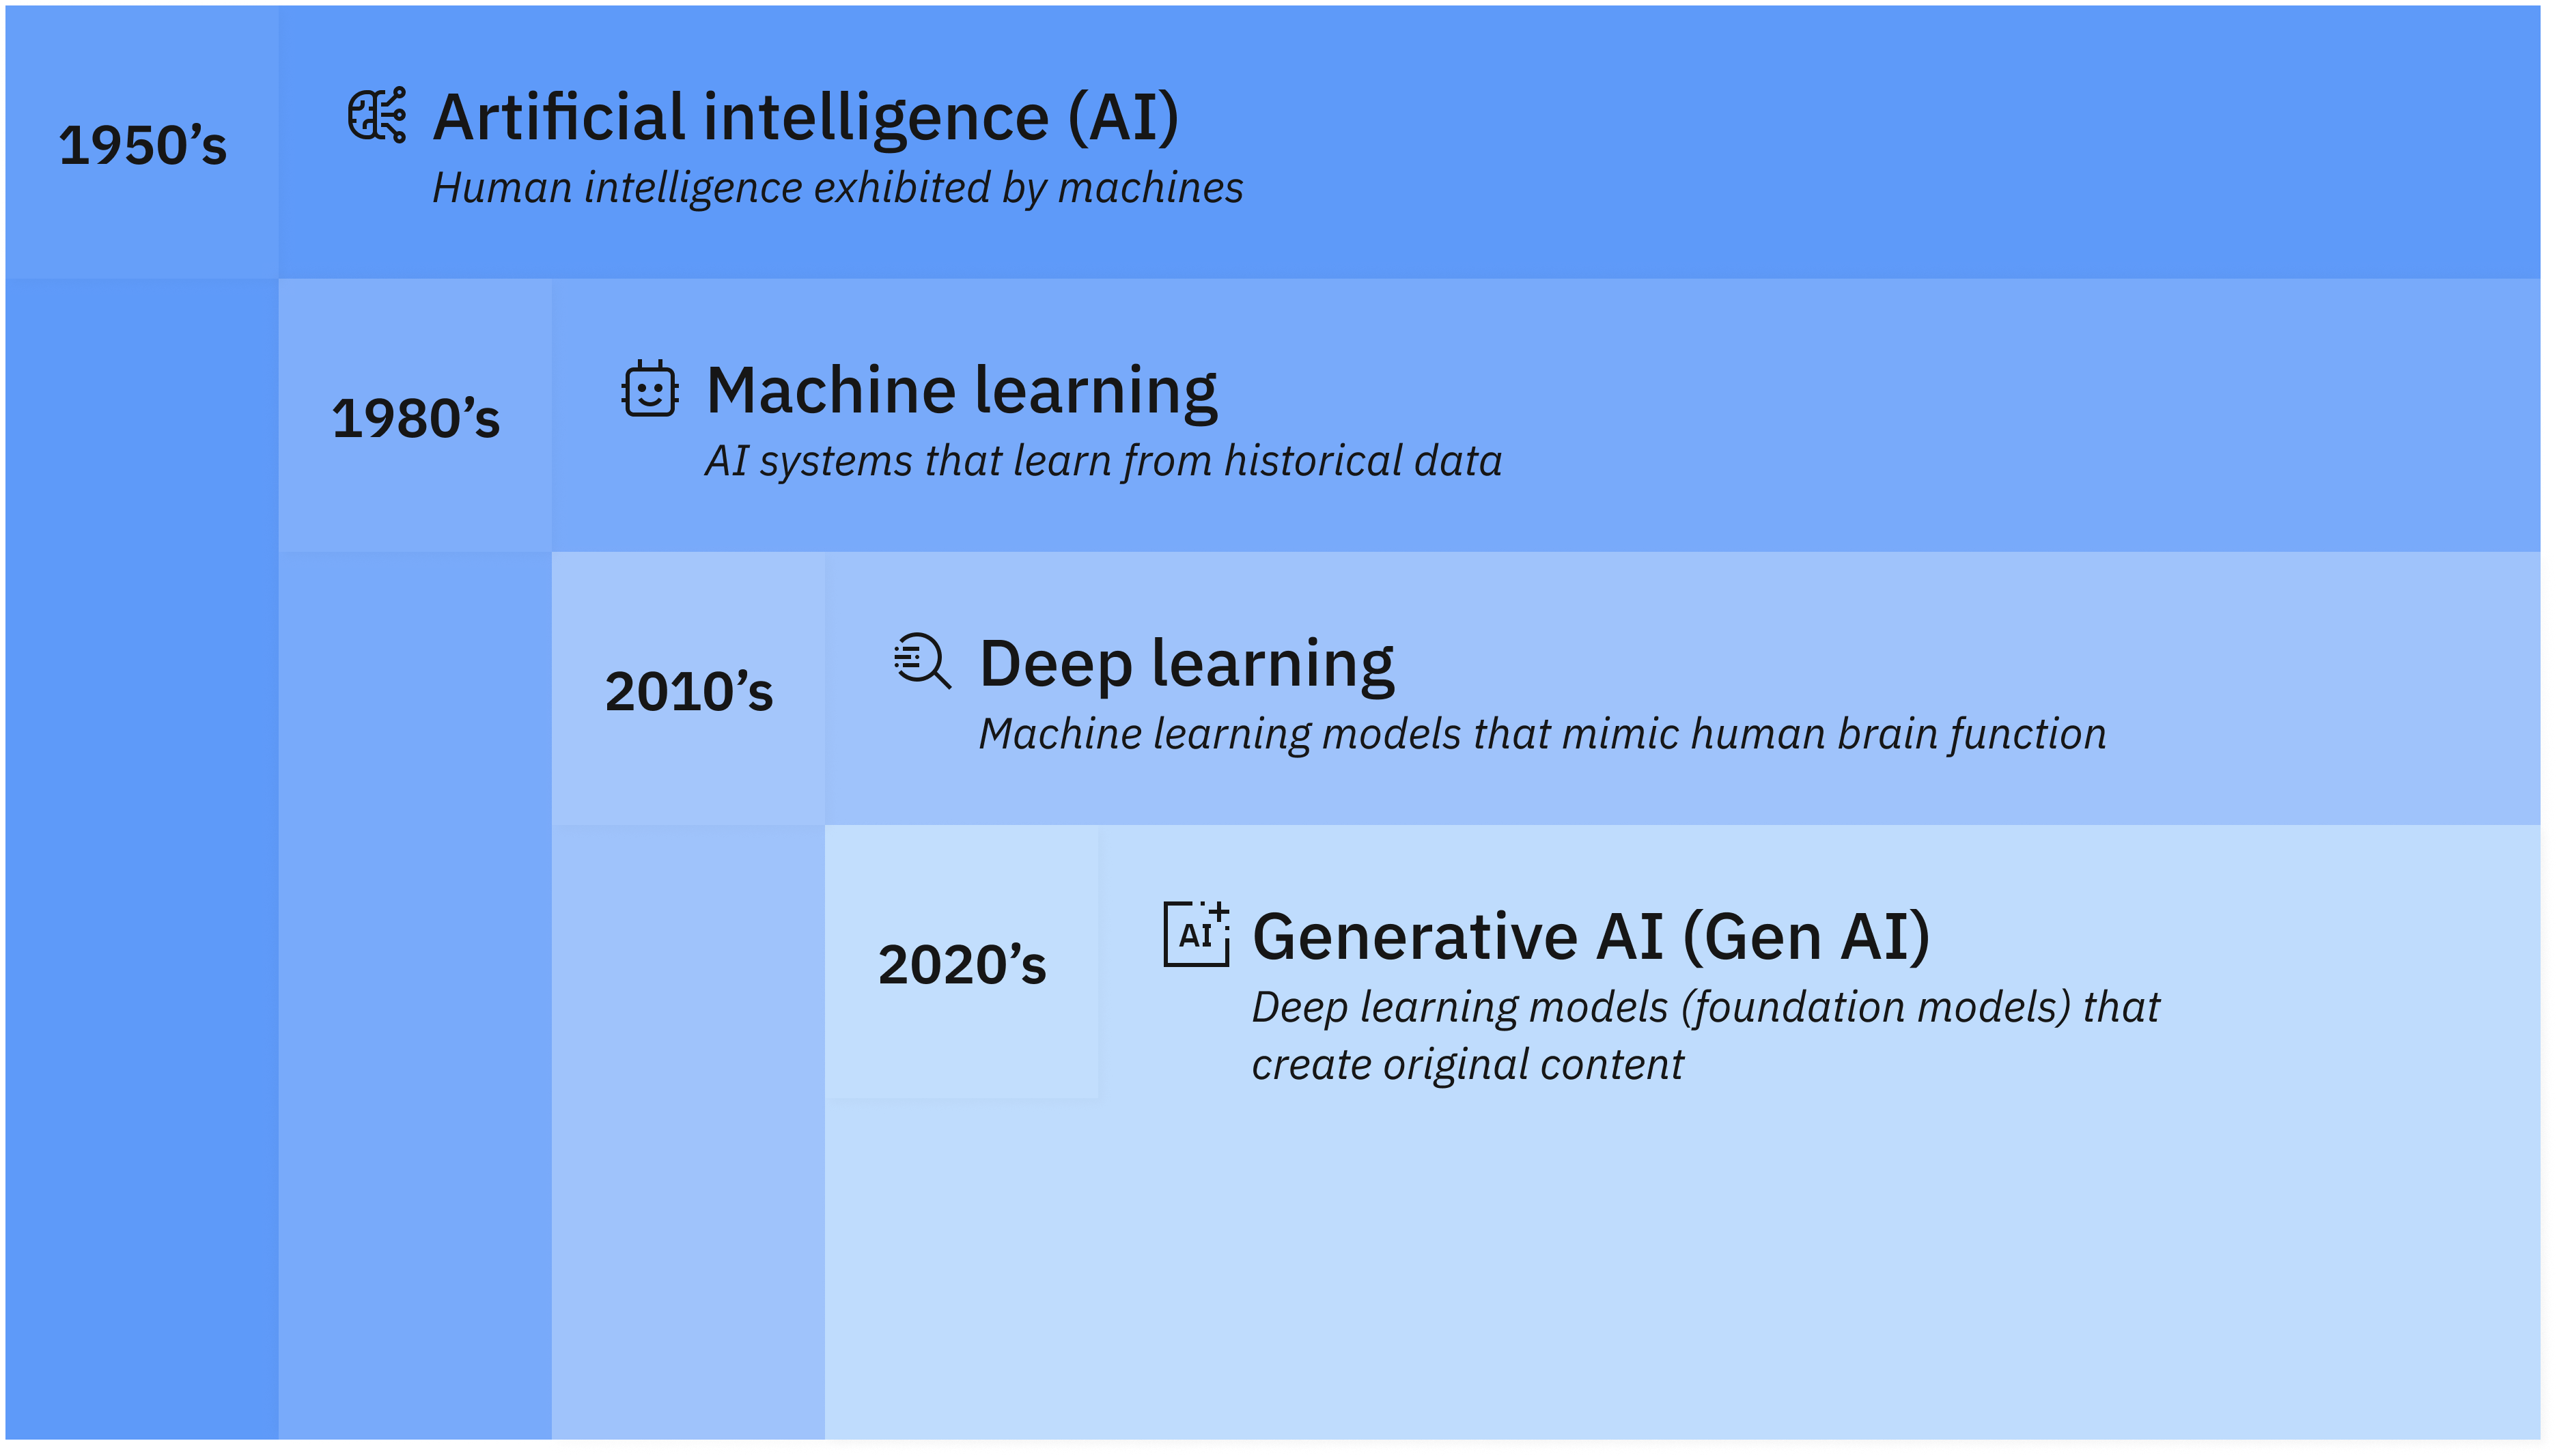
\includegraphics[alt={Diagramma dei concetti racchiusi nalla scienza dell'AI}, width=1\columnwidth]{img/diagram-ai-ml-dl-genai.png}
    \caption{Diagramma dei concetti racchiusi nell'IA rilevanti per questa tesi}
    \label{fig:diagram-ai-sub-concepts}
\end{figure}

Considerata la natura del progetto svolto in stage e lo scopo di questo documento, approfondirò in questa tesi solo i temi pertinenti affrontati durante il progetto. Tuttavia, è sufficiente soffermarsi un momento e osservare il mondo che ci circonda per rendersi conto di come l'IA sia ormai una parte integrante della nostra vita quotidiana: dalla medicina all'automazione industriale, dalla finanza al riconoscimento vocale e visivo, dai motori di ricerca agli algoritmi di suggerimento dei contenuti sui social networks. I contesti di applicazione sono innumerevoli e le possibili aree di discussione sono vastissime.


\subsection{Apprendimento Automatico}

Direttamente sotto ad IA, abbiamo l'Apprendimento Automatico, meglio noto come \textit{Machine Learning(ML)} in inglese. È il sotto-insieme che si occupa di sviluppare modelli a partire da algoritmi ai quali vengono forniti dati affinché possano apprendere e migliorare la loro performance a un determinato compito, per esempio riconoscere pattern o fare previsioni su nuovi dati. \\
Normalmente per la risoluzione di un problema si ricorre all'approccio classico, sviluppando un algoritmo e scrivendo un programma in grado di risolverlo. Tuttavia in alcuni casi questo metodo non è utilizzabile per svariate ragioni:
\begin{itemize}
    \item \textbf{impossibile formalizzare il problema} e quindi formulare un algoritmo di risoluzione;
    \item i dati sono affetti da \textbf{rumore e/o incertezza};
    \item \textbf{alto livello di complessità} nella formulazione della soluzione;
    \item \textbf{mancanza dei dati} che permetterebbero l'applicazione degli algoritmi tradizionali.
\end{itemize}

\begin{figure}[H]
    \centering
    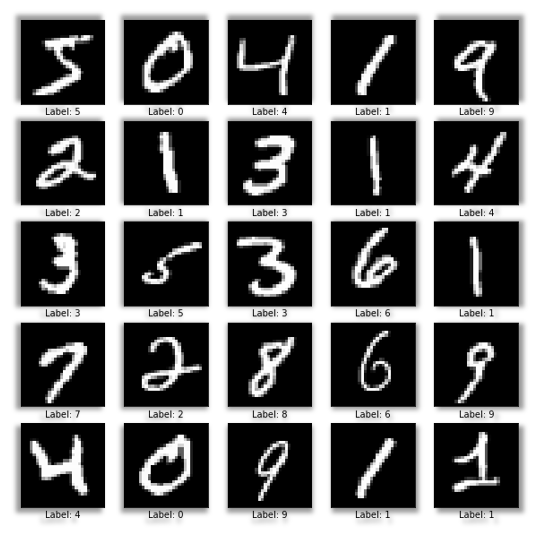
\includegraphics[alt={Numeri scritti a mano}, width=1\columnwidth]{img/handwritten-digit-recognition.png}
    \caption{Numeri scritti a mano}
    \label{fig:digit-recognition}
\end{figure}

L'esempio classico di problema dove non è possibile applicare algoritmi tradizionali è, come si vede in Figura \ref{fig:digit-recognition} quello del riconoscimento di numeri scritti manualmente, dove è appunto molto difficile formalizzare il problema, i dati possono essere ambigui e sfocati.\\

Vi sono 3 categorie principali di algoritmi di ML, come illustrato in Figura \ref{fig:ml-paradigms}.

\begin{figure}[H]
    \centering
    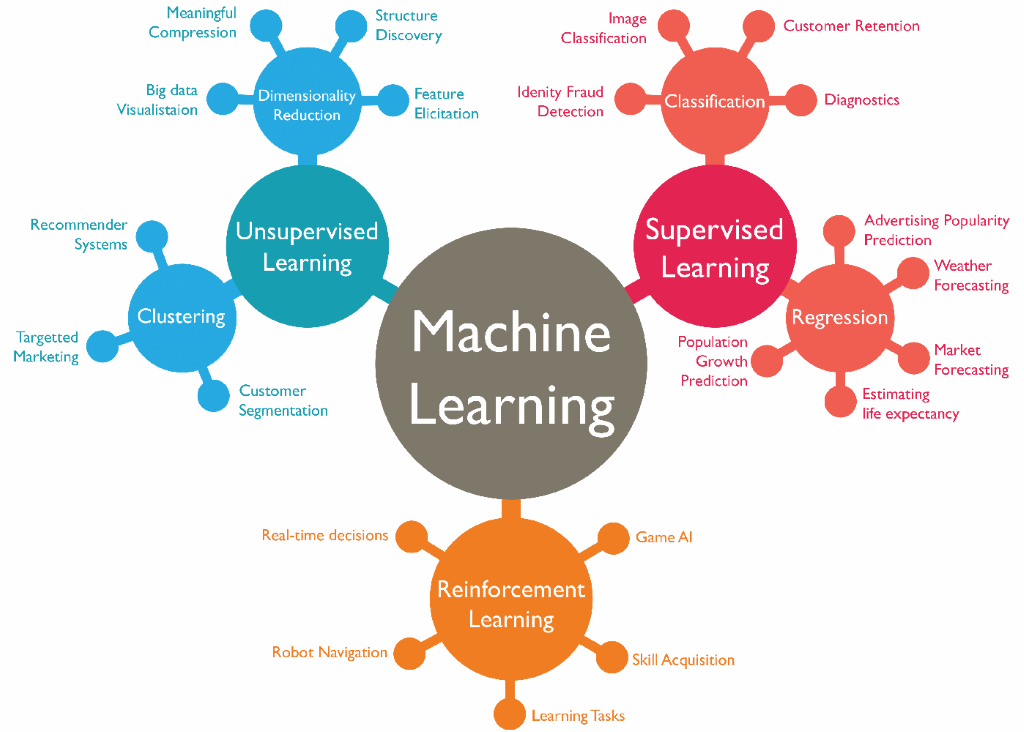
\includegraphics[alt={Suddivisione classica dei paradigmi di apprendimento nel ML}, width=1\columnwidth]{img/paradigmi-ml.png}
    \caption{Suddivisione classica dei paradigmi di apprendimento nel ML}
    \label{fig:ml-paradigms}
\end{figure}

\subsubsection{Supervised Learning}

Gli algoritmi di \textit{Supervised Learning(SL)} sono i più utilizzati. Con questo modello, un \textit{data scientist} agisce da guida e insegna all'algoritmo i risultati da generare. Esattamente come un bambino impara a identificare i frutti memorizzandoli in un libro illustrato, nel ML supervisionato l'algoritmo apprende da un set di dati già etichettato e con un output predefinito.

Gli algoritmi di regressione lineare e logistica, di classificazione multiclasse e le macchine a vettori di supporto sono alcuni esempi di apprendimento automatico supervisionato.

\subsubsection{Unsupervised Learning}

Lo \textit{Unsupervised Learning(UL)} utilizza un approccio più indipendente, in cui un computer impara a identificare processi e schemi complessi senza la guida attenta e costante di una persona. L'apprendimento automatico non supervisionato implica una formazione basata su dati privi di etichette e per i quali non è stato definito un output specifico.

Per continuare a utilizzare l'analogia precedente, il ML non supervisionato è simile a un bambino che impara a identificare i frutti osservando i colori e gli schemi, anziché memorizzando i nomi con l'aiuto di un insegnante. Il bambino cercherà le somiglianze tra le immagini e le suddividerà in gruppi, assegnando a ciascun gruppo la nuova etichetta corrispondente. Gli algoritmi di \textit{clustering k-means}, l'analisi di componenti principali e indipendenti e le regole di associazione sono esempi di UL.

\subsubsection{Reinforcement Learning}

Il \textit{Reinforcement Learning(RL)}, o apprendimento per rinforzo, ha come obiettivo la realizzazione di modelli che siano in grado di decidere in autonomia la prossima migliore azione da svolgere interagendo con l'ambiente in cui si trovano. Questo paradigma dell'apprendimento automatico si differenzia da quello della SL nel \textit{dataset} utilizzato per l'apprendimento: i dati forniti non possiedono etichette e output, sarà l'algoritmo stesso che deciderà cosa fare in base allo stato attuale del sistema. Mentre nella ML supervisionato la decisione viene presa all'inizio quando si riceve il dato, nel caso della RL le decisioni vengono prese sequenzialmente, in base allo stato input corrente.

Gli algoritmi utilizzati dalla RL imparano dall'output della propria azione, andando a tentativi: ognuno di questi fornisce un feedback positivo-negativo-neutro che permette all'algoritmo RL di determinare se l'azione intrapresa fosse corretta, con lo scopo finale di massimizzare le ricompense con ciascuna decisione.
Esempi di algoritmi di \textit{Reinforcemente Learning} sono il \textit{Q-learning}, \textit{Proximal Policy Optimization} e il \textit{Deep Q-Network}.


\subsection{Natural Language Processing}

La \textit{Natural Language Processing(NLP)} è anch'essa una sottobranca dell'Informatica e dell'Intelligenza Artificiale che utilizza l'Apprendimento Automatico per ottenere modelli in grado di capire e comunicare con il linguaggio umano.
La NLP consente a computer e dispositivi digitali di riconoscere, comprendere e generare testo e discorsi, combinando la linguistica computazionale, ovvero la modellazione delle regole della lingua umana, con la modellazione statistica, l'apprendimento automatico (ML) e il \textit{deep learning}, campo di ricerca dell'apprendimento automatico e dell'AI che sviluppa modelli il cui funzionamento simula il cervello umano, formando delle reti neurali artificiali organizzate in diversi strati, dove ogni strato calcola i valori per quello successivo affinché l'informazione venga elaborata in maniera sempre più completa.

La ricerca sulla NLP ha aperto la strada all'era dell'Intelligenza Artificiale Generativa, dalle capacità comunicative dei modelli di linguaggio di grandi dimensioni (LLM) alla capacità dei modelli di generazione di immagini di comprendere le richieste. La NLP è già parte della vita quotidiana per molti, alimentando motori di ricerca, attivando chatbot per il servizio clienti con comandi vocali, sistemi GPS a comando vocale e assistenti digitali su \textit{smartphone}.

La NLP svolge anche un ruolo sempre più importante nelle soluzioni aziendali che aiutano a semplificare e automatizzare le operazioni aziendali, aumentare la produttività dei dipendenti e semplificare i processi aziendali critici.


\subsection{AI Generativa}

La \textit{Generative AI}, talvolta chiamata semplicemente \textit{Gen AI}, sono algoritmi di \textit{deep learning} in grado di generare contenuto originale come testi, codice, immagini, video e audio a partire da un prompt umano, ovvero un testo dove l'utente descrive la propria richiesta su cosa vorrebbe ottenere dalla \textit{Gen AI}. \\

\begin{figure}[H]
    \centering
    
\includegraphics[alt={Logo di ChaGPT GPT-3.5}, width=0.3\columnwidth]{img/gpt-3-5-logo.png}
    \caption{Logo di GPT-3.5}
    \label{fig:gpt-logo}
\end{figure}

Negli ultimi anni, è proprio questo il campo dell'IA che ha ricevuto maggiore attenzione grazie all'arrivo della versione GPT-3.5 di ChatGPT nel 2022 (\ref{fig:gpt-logo}), modello sviluppato dall'azienda OpenAI che con la sua capacità di comprendere e generare testo in modo estremamente naturale e coerente ha riportato interesse sull'argomento delle AI in generale. Infatti a partire da allora si è potuto osservare una diffusa adozione della tecnologia in svariati settori tra cui lo sviluppo software, il marketing, la moda e la farmaceutica solo per citarne alcuni.
La versatilità in molteplici ambiti, combinata ad una comprensione del linguaggio naturale quasi "umana", ha fatto sì che le persone vedessero nuove possibilità di automazione, creatività assistita e miglioramento delle interazioni uomo-macchina.\\

Alla base, un modello di \textit{Gen AI} viene realizzato in 3 fasi: 
\begin{enumerate}
    \item \textbf{addestramento}: per prima cosa si addestra un algoritmo di \textit{deep learning} su un'enorme quantità di dati grezzi producendo un \textit{foundation model}, una rete neurale con miliardi di parametri in grado di generare contenuti autonomamente in risposta ai prompt; si tratta di un processo ad alta intensità computazionale, costoso e che necessita  settimane di elaborazione da parte di migliaia di unità di elaborazione grafica (GPU) in \textit{cluster};
    \item \textbf{tuning}: il modello di base ottenuto è generalista, per migliorarlo nella generazione di uno specifico argomento o compito si ricorre al \textit{Fine-Tuning}, processo in cui si forniscono dati etichettati specifici per l'applicazione, come possibili domande che potrebbe incontrare e la relativa risposta corretta che si aspetta;
    \item \textbf{generazione, valutazione risultati e ulteriore tuning}: sviluppatori e utenti valutano regolarmente i risultati del modello IA generativo e continuano il processo di \textit{fine-tuning} per ottenere una maggiore accuratezza.
\end{enumerate} 


\newpage
\subsection{Large Language Model}
\subsubsection{Introduzione}
I modelli di linguaggio di grandi dimensioni, in inglese \textit{Large Language Model(LLM)}, sono i \textit{foundation model} attualmente più diffusi, addestrati su enormi \textit{dataset} testuali, usando spesso risorse web come Wikipedia e Github, appositamente per il compito di generazione di testi. \\

Sono in grado di fare questo perché attraverso il processo di addestramento, hanno imparato i vari significati che assume ciascuna parola, basandosi sul fatto se viene usata singolarmente o assieme ad altre e il contesto in cui si trova. Per esempio sono in grado di capire quando la parola "tirare" significa il contrario di spingere se riguardo una porta o lanciare un oggetto. \\

Alla base di questi modelli sta l'architettura di rete neurale \textbf{\textit{Transformers}}: a differenza di quelle tradizionali, utilizza il meccanismo di "attenzione", ovvero vi sono neuroni specifici che sono in grado di influenzare sugli altri in modo da determinare la parte più importante in una sequenza di dati, il che le rende perfette per l'elaborazione dei linguaggi data la natura sequenziale dei dati testuali. 
Questo permette ai modelli di:
\begin{itemize}
    \item elaborare intere sequenze di dati, quindi frasi intere invece che solo singole parole, in modo simultaneo;
    \item comprendere il contesto di una sequenza di dati;
    \item codificare i dati in \textit{embeddings}, ovvero vettori numerici che rappresentano il loro significato e il contesto.
\end{itemize}
Oltre a velocizzare il processo di addestramento, i modelli \textit{transformers} sono perfetti per i compiti di \textit{Natural Language Processing(NLP)} e \textit{Natural Language Understanding(NLU)}, rendendogli in grado di generare testi molto più lunghi in risposta a domande, ma anche poesie o articoli scientifici, il tutto in modo più accurato. 

\subsubsection{Prompt Engineering}
Un \textit{prompt} è un testo in linguaggio naturale che viene fornito al modello AI e descrive il compito che deve svolgere.
Nel caso della generazione di testo, può limitarsi ad una semplice domanda come "Cos'è la Generative AI?", un comando del tipo "Genera una storia ambientata durante il Medioevo", oppure una descrizione testuale più lunga contenente informazioni aggiuntive sul contesto, degli esempi da seguire, la struttura della risposta, oppure è possibile assegnare un ruolo che il modello dovrà rispettare e simulare, ad esempio "Parlami come se fossi un legionario romano del Tardo Impero".

Lo scopo del \textit{Prompt Engineering} è quello di strutturare il prompt in modo da guidare il modello di AI generativa affinché riesca a comprendere la richiesta ed ottenere i risultati sperati. Sebbene cerchino di imitare gli esseri umani, richiedono istruzioni dettagliate per creare risultati pertinenti e di alta qualità. Quando si scrive un prompt, affinché l'IA Generariva di un'applicazione funzioni come previsto, è necessario utilizzare la creatività unita a tentativi ed errori per creare una raccolta di testi di input.

\subsubsection{Limitazioni e rischi}
Nonostante i modelli linguistici di grandi dimensioni siano molto flessibili e possano svolgere diverse attività come riassumere documenti, completare frasi, rispondere a domande e tradurre lingue, rimangono una tecnologia con le sue limitazioni e rischi che vanno tenuti conto: 
\begin{itemize}
    \item \textbf{allucinazioni e output imprecisi}: i modelli possono generare risposte che sembrano plausibili, ma sono in realtà prive di senso e/o completamente inventate;
    \item \textbf{mancanza di trasparenza}: i modelli operano spesso come delle \textit{black boxes}, rendendo difficile capire in che modo sono arrivati a generare l'\textit{ouput};
    \item \textbf{possibile bias}: i modelli potrebbero essere influenzati da bias originati dai contenuti utilizzati come dati di addestramento o durante il processo di \textit{fine-tuning};
    \item \textbf{costo computazionale elevato}: i LLM più performanti necessitano di un'elevata potenza di calcolo computazione per funzionare in modo efficiente, altrimenti la generazione di output può richiedere molto tempo, aumentando di conseguenza i costi;
    \item \textbf{sicurezza}: i modelli possono essere utilizzati per scopi malefici come la generazione di mail di truffa, false identità o altro contenuto con fine nocivo;
    \item \textbf{sicurezza e privacy dei dati}: durante la fase di training o la stesura dei prompt, bisogna fare attenzione a non utilizzare informazioni riservate o tutelate da diritti di proprietà intellettuale.
\end{itemize}


\subsection{Retrieval Augmented Generation}

\subsubsection{Introduzione}
La \textit{Retrieval Augmented Generation(RAG)} è una tecnica di ricerca di informazioni utilizzata principalmente per aiutare i LLMs nel loro processo di generazione, ampliando il loro dominio conoscitivo fornendo informazioni inerenti al contesto applicativo e alla richiesta umana o semplicemente dati più recenti ed aggiornati che sicuramente i modelli non possiederebbero perché non presenti nel loro \textit{dataset} di addestramento. \\
Utilizzata assieme a tecniche di \textit{prompt engineering} come l'utilizzo di \textit{guardrail}, ovvero regole e restrizioni impostate al modello su quali fonti utilizzare, è una possibile soluzione per mitigare il rischio di generare allucinazioni e risposte imprecise da parte dell'AI in quanto gli vengono forniti dati affidabili e pertinenti alla richiesta.
Inoltre la RAG è un approccio molto conveniente in quanto estende le capacità già avanzate degli LLM a domini specifici o alla sua conoscenza di base, permettendogli di continuare ad essere pertinente, accurato e utile in vari contesti, il tutto senza la necessità di svolgere \textit{fine-tuning}.

\subsubsection{Funzionamento}
\begin{figure}[H]
    \centering
    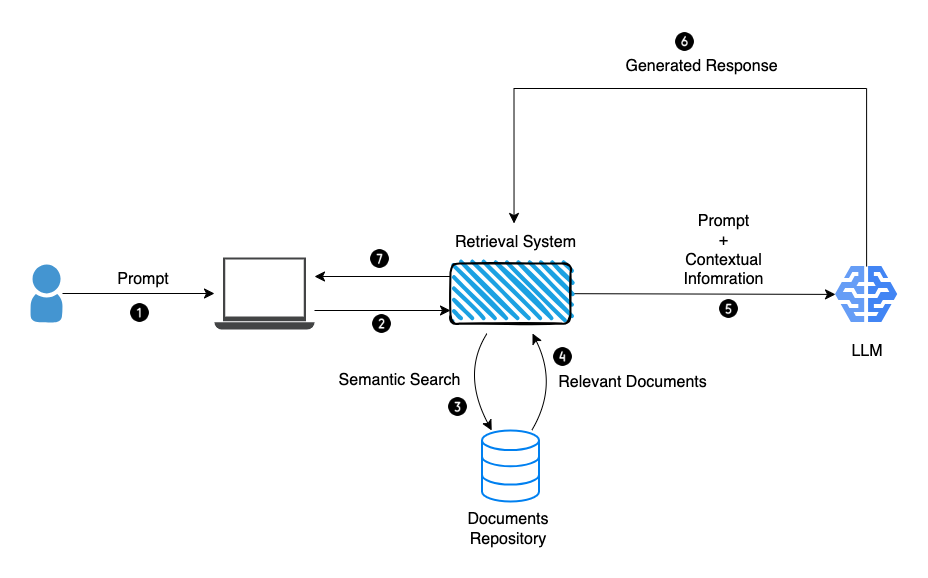
\includegraphics[alt={Diagramma funzionamento della RAG}, width=1\columnwidth]{img/diagram-rag.png}
    \caption{Passaggi della Retrieval Augmented Generation}
    \label{fig:rag-diagram}
\end{figure}

Come da Figura \ref{fig:rag-diagram} il processo della RAG si suddivide in tre fasi principali: \textit{Data Ingestion}, \textit{Retrieval} e \textit{Generation}.

\paragraph*{Data Ingestion}
Durante questa prima fase viene composto il \textit{dataset} contenente le informazioni aggiuntive riguardanti il contesto di applicazione: dati esterni al set di training vengono processati in base al loro formato, poi saranno convertiti in vettori di \textit{embedding}, rappresentazioni numeriche del contenuto testuale di partenza, per essere finalmente salvati all'interno di database vettoriali, pronti all'uso.
Il compito di generare questi vettori numerici è generalmente assegnato a modelli AI specializzati, noti come \textit{Embedding Model}.

\paragraph*{Information Retrieval}
Una volta che l'utente scrive la sua richiesta nel prompt, questa viene utilizzata per svolgere la ricerca vettoriale all'interno del database: lo stesso modello di Embedding usato durante la \textit{Data Ingestion} genera il vettore numerico a partire dalla \textit{query} umana.\\
Questo verrà impiegato per la ricerca vettoriale all'interno della base di dati al fine di recuperare le informazioni più inerenti archiviate nel \textit{vector store}: più precisamente viene calcolata la similarità semantica specificata, nel caso del progetto di stage questa era la \textit{Cosine Similarity}, cioè il coseno dell'angolo che intercorre tra il vettore della \textit{query} e quelli salvati nello spazio multidimensionale.\\
Dati due vettori di attributi numerici, A e B, il livello di similarità tra di loro è espresso utilizzando la formula:

\[
\text{Cosine Similarity}(\mathbf{A}, \mathbf{B}) = \cos(\theta) = \frac{\mathbf{A} \cdot \mathbf{B}}{\|\mathbf{A}\| \|\mathbf{B}\|} 
\]

dove \begin{math}\theta\end{math} è l'angolo tra i due vettori.
Il valore calcolato viene utilizzato per determinare la similarità semantica dei testi originali rappresentati dai vettori: questo numero può variare da +1, semanticamente simili con contesto o tematiche in comune, a 0, significato distaccato e mancanza di alcuna relazione tra i contenuti affrontati.

\paragraph*{Generation}
Una volta recuperate le informazioni inerenti dal database, queste vengono aggiunte nel prompt originale dell'utente in modo da consentire al LLM di generare una risposta accurata alla richiesta dell'utente. \\
È importante scrivere i prompt in modo intelligente, fornendo istruzioni sul \textit{task} da svolgere in modo chiaro e conciso e organizzando i dati inerenti in modo strutturato così da facilitare la comprensione al modello.

\subsection{Embedding}
L'Incorporamento, in inglese \textit{Embedding}, è un mezzo per rappresentare oggetti come testo, immagini e audio come punti in uno spazio vettoriale continuo, in cui le posizioni di tali punti nello spazio sono semanticamente significative per gli algoritmi di ML.\\
Per il funzionamento del processo della Retrieval Augmented Generation, l'incorporamento è una parte fondamentale in quanto permette di trovare oggetti semanticamente simili alle richieste dell'utente in modo rapido e senza dover dipendere da campi stringa o corrispondenze di parole chiave.\\
Gli oggetti che entrano in un modello di \textit{Embedding} vengono emessi come incorporamenti, o \textit{embeddings}, rappresentati come vettori. Ognuno di questi è una serie di numeri (ad es. [56, 222… 3, 7272] ), in cui ciascun numero indica dove si trova un oggetto lungo una dimensione specificata. Il numero di dimensioni può raggiungere un migliaio o più, a seconda della complessità dei dati di input e il modello di Embedding utilizzato. Più un vettore è vicino ad altri in questo spazio n-dimensionale, più saranno simili. La somiglianza di distribuzione è determinata dalla lunghezza dei punti vettoriali da un oggetto all'altro e può essere misurata in diversi modi, per esempio \textit{Cosine Similarity}, \textit{Euclidean Distance} e \textit{Manhattan Distance}.

 
\newpage
\section{Linguaggi di programmazione}
Come linguaggi di programmazione utilizzati durante il progetto vi sono Typescript e Python, rispettivamente per le due versioni dell'assistente sviluppate. La scelta dei due linguaggi è stata imposta dal tutor aziendale in base alle librerie obbligatorie da utilizzare per sviluppare le rispettive versioni.

\subsection{Typescript}
\textbf{Typescript(TS)} è uno dei linguaggi di programmazione più utilizzati al giorno d'oggi. Spesso definita come una "variante" di \textbf{Javascript(JS)}, linguaggio da cui deriva e con cui presenta una relazione particolare.\\
Javascript era nato inizialmente come un semplice linguaggio di \textit{scripting} per \textit{browser} per scrivere poche linee di codice da incorporare all'interno di pagine web. Con la crescita esponenziale dell'uso di Internet, inizialmente concepito come semplice insieme di pagine statiche, ma ormai trasformata in una piattaforma per applicazioni di qualsiasi tipo, anche Javascript ha avuto un'evoluzione parallela. Da linguaggio semplice e limitato, è diventato sempre più popolare e sofisticato, ampliando enormemente le possibilità di sviluppo, al punto da essere utilizzata anche al di fuori del contesto applicativo dei \textit{browsers}, come l'implementazione di server JS utilizzando \textit{node.js}.\\
Quindi essendo nato come linguaggio per l'uso veloce e semplice, mentre ora è uno strumento versatile per sviluppare applicazioni con migliaia di righe, è normale che vi siano delle sorprese inaspettate:
\begin{itemize}
    \item l'operatore di uguaglianza (\verb|==|) converte automaticamente i suoi operandi, causando comportamenti inattesi:
    \begin{listing}[H]
        \begin{minted}[bgcolor=lightgray]{js}
        if ("" == 0) {
        // Vero, ma perché?? }
        if (1 < x < 3) {
        // Vero per *qualsiasi* valore di x!}
        \end{minted}
        \caption{Esempio di errore JS con operatore di uguaglianza ==}
        \label{listing:js-error-1}
    \end{listing}
    \item JS permette di accedere ad attributi non esistenti:
    \begin{listing}[H]
        \begin{minted}[bgcolor=lightgray]{js}
        const obj = { larghezza: 10, altezza: 15 };
        const area = obj.larghezza * obj.altteza;
        // Perché NaN(Not a Number)? Errore di battitura!
        \end{minted}
        \caption{Esempio di errore JS con accesso ad attributo inesistente}
        \label{listing:js-error-2}
    \end{listing}
\end{itemize}
In questi casi la maggior parte dei linguaggi di programmazione avrebbe segnalato un errore.\\
\textbf{Typescript} è stato sviluppato proprio per evitare questo genere di problemi in quanto svolge un "controllo statico dei tipi" prima di eseguire il codice al fine di trovare errori di "tipo".
TS è un "sovrainsieme tipizzato" di JS, il che significa che ogni programma JavaScript valido è anche un programma TypeScript valido in quanto mantiene la compatibilità con il codice JS esistente, tuttavia aggiunge un sistema di tipi opzionali consentendo di specificare i tipi di variabili, funzioni, e altri elementi del codice, il che aiuta a rilevare errori durante la fase di compilazione anziché a \textit{runtime}.\\
Durante lo stage, il \textit{backend} dell'assistente per Jira è stato sviluppato interamente in TypeScript. 

\subsection{Python}
\textbf{Python} è uno dei linguaggi di programmazione più usati al mondo. Grazie alla sua sintassi asciutta e potente, ed al supporto multi piattaforma, è utilizzato per moltissime tipologie di applicazioni, dal \textit{networking}, al web, fino al ML.
Tra i suoi punti di forza spuntano:
\begin{itemize}
    \item è \textbf{multi-paradigma}, supportando sia la programmazione procedurale (funzioni), sia la programmazione ad oggetti (ereditarietà singola e multipla, overloading degli operatori, duck typing) e anche diversi elementi della programmazione funzionale (come iteratori e generatori);
    \item è \textbf{portatile} in quanto linguaggio interpretato, quindi il codice può essere eseguito su qualsiasi piattaforma purché abbia l’interprete Python installato;
    \item è \textbf{facile da usare} dato che la sintassi e i diversi moduli e funzioni già inclusi nel linguaggio sono consistenti, intuitivi e facili da imparare;
    \item è \textbf{ricco di librerie} che possono essere scaricate attraverso il \textit{Python Package Index}, consentendo di utilizzare migliaia di moduli aggiuntivi creati e mantenuti dalla comunità.
\end{itemize}

All'interno del progetto di stage, la versione chatbot dell'assistente è stato sviluppato interamente con Python, sia il \textit{frontend} che il \textit{backend}.

\section{Tecnologie utilizzate}

\subsection{AWS Bedrock}

\subsubsection{Introduzione}
\textbf{AWS Bedrock} è una piattaforma completamente gestita che offre una varietà di modelli AI di grandi dimensioni da diversi provider, tra cui Amazon e aziende terze come AI21 Labs, Anthropic e Stability AI. Permette agli sviluppatori di scegliere il modello più adatto alle loro esigenze e di integrarlo facilmente nelle loro applicazioni.

\subsubsection{Funzionalità e vantaggi}
\begin{itemize}
    \item \textbf{\textit{Accesso a diversi modelli}}: testo, immagini, audio ed \textit{embedding};
    \item \textbf{personalizzazione}: possibilità di adattare i modelli ai propri dati e casi d’uso specifici;
    \item \textbf{scalabilità}: gestione automatica delle risorse per adattarsi alle esigenze di elaborazione.
\end{itemize}

\subsubsection{Casi d'uso}
AWS Lambda è adatto per una vasta gamma di casi d’uso, tra cui:
\begin{itemize}
    \item \textbf{\textit{generazione di testo}}: creazione di testo coerente e pertinente per risposte automatiche;
    \item \textbf{analisi di immagini}: estrazione di informazioni da immagini per supportare le risposte;
    \textit{elaborazione di audio}: trascrizione e analisi di file audio per risposte basate su contenuti multimediali.
\end{itemize}

\subsubsection{Utilizzo nel progetto}
Nel contesto del progetto, AWS Bedrock viene impiegato per due funzioni chiave:
\begin{enumerate}
    \item \textit{generazione di testo}: i modelli di linguaggio avanzati di AWS Bedrock sono utilizzati per produrre risposte automatiche coerenti e pertinenti ai ticket. Questo approccio migliora significativamente l’efficienza e la qualità del supporto tecnico, consentendo la creazione di proposte di soluzioni basate sul contesto storico dei ticket presenti nel sistema.
    \item \textit{generazione di \textit{embedding}}: i modelli specializzati di AWS Bedrock vengono sfruttati per generare rappresentazioni vettoriali (\textit{embedding}) dei dati testuali. Questa tecnica permette di effettuare analisi semantiche avanzate e di implementare funzionalità di ricerca e raccomandazione più sofisticate.
\end{enumerate}
L’integrazione di AWS Bedrock nel flusso di lavoro ottimizza i processi di gestione dei ticket, potenzia le capacità di analisi dei dati e contribuisce a un’esperienza di supporto più rapida e accurata per gli utenti.

\subsection{AWS Lambda}

\subsubsection{Introduzione}
\textbf{AWS Lambda} è un servizio \textit{serverless} di \textit{Amazon Web Services (AWS)} che consente di eseguire codice senza la necessità di gestire server o infrastrutture sottostanti. Le funzioni Lambda vengono eseguite in risposta a eventi specifici, garantendo scalabilità automatica e costi ridotti.

\subsubsection{Funzionalità e vantaggi}
\begin{itemize}
    \item \textbf{\textit{Serverless computing}}: offre un’infrastruttura \textit{serverless} per l’esecuzione di codice, eliminando la necessità di gestire server e risorse sottostanti;
    \item \textbf{scalabilità automatica}: le funzioni Lambda vengono scalate automaticamente in base al carico di lavoro, garantendo prestazioni elevate anche con picchi di traffico;
    \item \textbf{costi ridotti}: addebita solo per il tempo effettivo di esecuzione delle funzioni, riducendo i costi operativi rispetto all’utilizzo di server tradizionali;
    \item \textbf{integrazione con servizi AWS}: le funzioni Lambda possono essere integrate con altri servizi AWS, come API Gateway, S3 e DynamoDB, facilitando lo sviluppo di applicazioni complesse e scalabili;
    \item \textbf{monitoraggio e \textit{logging}}: fornisce strumenti integrati per il monitoraggio delle funzioni, inclusi i registri di esecuzione e le metriche di performance.
\end{itemize}


\subsubsection{Casi d'uso}
AWS Lambda è adatto per una vasta gamma di casi d’uso, tra cui:
\begin{itemize}
    \item \textbf{elaborazione di eventi}: le funzioni Lambda possono essere utilizzate per elaborare eventi in tempo reale, come notifiche, aggiornamenti di database e processi di trasformazione dei dati;
    \item \textbf{backend per applicazioni \textit{web e mobile}}: è efficace come \textit{backend} per applicazioni \textit{web e mobile}, consentendo di creare API scalabili e performanti senza la necessità di gestire l’infrastruttura sottostante;
    \item \textbf{automazione dei processi}: le funzioni Lambda possono automatizzare processi complessi, come l’elaborazione di file, la generazione di \textit{report} e la gestione dei \textit{workflow}, migliorando l’efficienza operativa e riducendo i tempi di risposta.
\end{itemize}

\subsubsection{Utilizzo nel progetto}
 Nel contesto del progetto, AWS Lambda è utilizzato per l’implementazione delle funzioni Lambda che gestiscono l’elaborazione dei ticket e la generazione delle risposte. Le funzioni Lambda vengono attivate in risposta agli eventi generati dai \textit{webhook} di Jira, consentendo di analizzare i ticket e generare proposte di soluzioni in modo automatizzato e tempestivo.


\subsection{LangChain}

\subsubsection{Introduzione}
\textbf{LangChain} è un \textit{framework} utilizzato per facilitare lo sviluppo di applicazioni che utilizzino i modelli di linguaggio di grandi dimensioni, permettendo di sviluppare componenti intercambiabili. Molto utile per costruire applicazioni che richiedono il collegamento di modelli di linguaggio con dati esterni, come API, database, documenti, o per gestire conversazioni complesse e multi-turno. \\
Presenta due librerie separate, rispettivamente per Javascript e Python.\\
La versione utilizzata è la 0.2 in entrambi i casi.

\subsubsection{Funzionalità e vantaggi}
\begin{itemize}
    \item \textbf{integrazione con LLMs}: il \textit{framework} presenta una estensiva libreria di integrazioni, supportando un grande numeri di Modelli linguistici differenti, intercambiabili tra loro;
    \item \textbf{componenti modulari e personalizzabili}: fornisce componenti modulari che possono essere personalizzati e combinati per lo sviluppo;
    \item \textbf{integrazione con fonti di dati esterne}: supporta l’integrazione con diverse fonti di dati esterni, come database, API e servizi su \textit{cloud}.
\end{itemize}

\subsubsection{Casi d'uso}
 Tra i casi d’uso di LangChain vi sono:
 \begin{itemize}
    \item \textbf{sviluppo di chatbot e assistenti virtuali}: utilizzato per lo sviluppo di Chatbot intelligenti e personalizzati che sono consapevoli del contesto e quindi in grado di rispondere a richieste complesse dell’utente in modo preciso e pertinente;
    \item \textbf{analisi dei sentimenti e delle opinioni}: le capacità di elaborazione del linguaggio naturale di Langchain possono essere utilizzate per analizzare i sentimenti e le opinioni espresse nei testi, come recensioni, commenti e feedback degli utenti;
    \item \textbf{Q\&A su documenti}: permette la creazione di applicazioni intelligenti con capacità di rispondere a domande su vaste quantità di documenti, sfruttando la tecnica della RAG.
\end{itemize} 

\subsubsection{Utilizzo nel progetto}
 Nel progetto le integrazioni di LangChain con MongoDB, Bedrock ed Ollama hanno permesso lo sviluppo di un assistente di supporto che genera in modo automatico delle proposte di risoluzione affidabili grazie all’utilizzo della tecnica della \textit{Retrival Augmented Generation}, recuperando documenti che trattano un problema simile a quello trattato nel ticket di supporto aperto.


\subsection{MongoDB}

\subsubsection{Introduzione}
\textbf{MongoDB} è un database NoSQL flessibile e scalabile, che supporta un modello di dati basato su documenti JSON e offre la capacità di effettuare ricerche vettoriali tramite la creazione di indici specializzati basati sui vettori di incorporamento generati da un modello di Embedding.\\

NoSQL, noto anche come "non solo SQL" o "non SQL", è un approccio alla progettazione di database che consente l'archiviazione e l'esecuzione di \textit{query} sui dati al di fuori delle strutture tradizionali presenti nei database relazionali.\\
Invece della tipica struttura tabellare di un database relazionale, i database NoSQL ospitano i dati all'interno di una struttura di dati, come un documento JSON. Non richiedendo uno schema, questo design di database non relazionale offre una rapida scalabilità per gestire insiemi di dati di grandi dimensioni e tipicamente non strutturati, rendendoli una scelta popolare tre le aziende odierne che hanno sempre più necessità di gestire grandi volumi di dati ad alta velocità e di scalare rapidamente per eseguire applicazioni web moderne in quasi tutti i settori.

\subsubsection{Funzionalità e vantaggi}
\begin{itemize}
    \item \textbf{modello di dati flessibile}: utilizza un modello di dati basato su documenti JSON, il quale permette di memorizzare dati con strutture variabili senza uno schema rigido;
    \item \textbf{scalabilità orizzontale}: è progettato per scalare orizzontalmente su cluster di server, gestendo carichi di lavoro distribuiti e garantendo prestazioni elevate anche con crescenti volumi di dati;
    \item \textbf{embedding}: supporta l'archiviazione di \textit{embeddings}, permettendo di effettuare ricerche vettoriali per ottenere risultati più precisi e pertinenti, inoltre consente il salvataggio dei vettori numerici direttamente all’interno di un campo di un documento, semplificando così la gestione e l’accesso ai dati.
    \item \textbf{ricerche vettoriali}: consente l’esecuzione di ricerche vettoriali mediante la creazione di indici specializzati basati sugli \textit{embedding} memorizzati nei documenti, permettendo di effettuare \textit{query} basate sulla similarità dei vettori, facilitando l’analisi dei dati e l’estrazione di informazioni pertinenti dalle collezioni di ticket;
    \item \textbf{integrazione con tecnologie \textit{cloud} e AI}: può essere facilmente integrato con le piattaforme \textit{cloud}, inclusa Amazon Web Services (AWS), facilitando l’utilizzo di servizi avanzati di intelligenza artificiale e l’elaborazione dei dati in tempo reale. Questa integrazione supporta la creazione di soluzioni scalabili e ad alte prestazioni, sfruttando i potenti strumenti di analisi e di elaborazione dei dati offerti dalle piattaforme \textit{cloud}.
\end{itemize}

\subsubsection{Casi d'uso}
MongoDB è adatto per una vasta gamma di casi d’uso, tra cui:
\begin{itemize}
    \item \textbf{gestione dei dati semi-strutturati}: MongoDB è ideale per la gestione di dati che non seguono uno schema fisso, come i documenti JSON;
    \item \textbf{analisi e query avanzate}: MongoDB consente di eseguire \textit{query} avanzate e analisi su grandi volumi di dati in modo efficiente;
\end{itemize}

\subsubsection{Utilizzo nel progetto}
\begin{figure}[H]
    \centering
    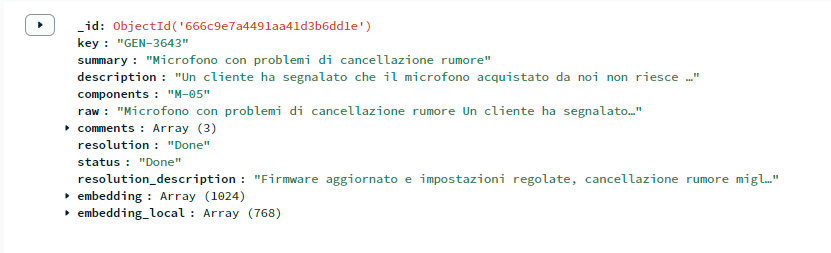
\includegraphics[alt={Esempio di documento salvato nel database}, width=1\columnwidth]{img/ticket_example.png}
    \caption{Esempio di ticket caricato nel database MongoDB}
    \label{fig:ticket-example}
\end{figure}

Nel contesto del progetto, MongoDB viene impiegato inizialmente per la memorizzazione dei ticket e delle risposte generate dal sistema. 
I ticket sono archiviati all’interno della collezione \textbf{tickets} come documenti JSON, come si può vedere in figura \ref{fig:ticket-example}, e possiedono due campi specifici per la memorizzazione dei vettori \textit{embedding} rispettivamente generati dal modello \textit{cloud} e quello locale.
Questo approccio permette di eseguire ricerche vettoriali, generando proposte di soluzioni basate sulla similarità con i ticket presenti nel sistema.\\
In seguito nella stesso database è stata realizzata una seconda collezione, denominata \textbf{feedbacks}, per salvare appunto i feedback lasciati dall’utente per migliorare le risposte del chatbot. Anche in questo caso ogni riscontro possiede un campo specifico dove è salvato il vettore numerico creato sulla domanda per la quale è stato lasciato. 
Per ogni risposta, il chatbot riceverà quindi, se presenti, anche i feedback più simili alla domanda ricevuta.


\subsection{Ngrok}

\subsubsection{Introduzione}
Servizio di \textit{reverse proxy server} utilizzato per stabilire una connessione sicura con la propria macchina (localhost), così da poter accedere da remoto al mio computer provvisto di scheda video NVIDIA sul quale operano, attraverso la piattaforma Ollama, i modelli locali.\\
La versione utilizzata è la 3.12.0.

\subsubsection{Funzionalità e vantaggi}
\begin{itemize}
    \item \textbf{\textit{Tunneling} sicuro e accesso remoto}: creazione di tunnel sicuri che permettono di esporre server locali a Internet;
    \item \textbf{autenticazione e sicurezza avanzata}: Ngrok permette di impostare l’autenticazione tramite \textit{token} e la crittografia dei tunnel per un maggiore grado di sicurezza;
    \textit{analisi e monitoraggio del traffico}: Ngrok fornisce una \textit{dashboard} e strumenti di analisi del traffico in tempo reale, permettendo agli sviluppatori di vedere richieste HTTP, analizzare \textit{payload}, e monitorare l’uso del servizio.
\end{itemize}

\subsubsection{Casi d'uso}
Tra i casi d’uso di Ngrok vi sono:
\begin{itemize}
    \item \textbf{dimostrazioni e presentazioni \textit{live}}: durante presentazioni o demo, gli sviluppatori possono utilizzare Ngrok per mostrare il funzionamento delle loro applicazioni ospitate localmente;
    \item \textbf{sviluppo e test di applicazioni web}: gli sviluppatori possono utilizzare Ngrok per esporre le loro applicazioni web in sviluppo su macchine locali, rendendole accessibili per svolgere test e ricevere feedback senza doverle distribuire su server pubblici.
\end{itemize}

\subsubsection{Utilizzo nel progetto}
 Ngrok nel progetto è stato utilizzato per stabilire una connessione sicura sulla porta locale 11343 della macchina avente in esecuzione Ollama, così da poter utilizzare da remoto, su un computer diverso, i modelli locali accelerati con una scheda video NVIDIA.

\subsection{Ollama}

\subsubsection{Introduzione}
\textbf{Ollama} è uno strumento AI avanzato che permette di utilizzare LLM in locale. Fornisce una piattaforma \textit{user-friendly} per installare, eseguire, gestire e personalizzare modelli di linguaggio di grandi dimensioni localmente. Viene eseguito su una porta locale del proprio computer.\\
La versione utilizzata corrisponde alla 0.2.5.

\subsubsection{Funzionalità e vantaggi}
\begin{itemize}
    \item \textbf{Esecuzione locale di LLM}: Ollama permette di installare ed eseguire modelli localmente, sfruttando le risorse del processore o, consigliato, della scheda video;
    \item \textbf{libreria estesa di modelli}: Ollama presenta una libreria contente un grande numero di LLM \textit{open-source} disponibili per l’installazione ed esecuzione. Inoltre è possibile importare modelli esterni, per esempio da Hugging Face, convertendoli al formato \textit{GPT Generated Unified Format (GGUF)};
    \item \textbf{\textit{user friendly}}: lo strumento possiede un’interfaccia semplice e facile da utilizzare, permettendo all’utente di eseguire il modello scelto in pochi passaggi;
    \item \textbf{compatibilità SO}: Ollama attualmente può essere usato sia su Mac che su Linux. Su Windows si può scaricare la \textit{preview} o ricorrere all'immagine Docker ufficiale su Docker Hub e utilizzarlo sul Sottosistema Windows per Linux.
\end{itemize}

\subsubsection{Casi d'uso}
Nella libreria di Ollama sono disponibili modelli per i compiti più svariati:
\begin{itemize}
    \item \textbf{generazione di testo}: creazione di testo coerente e pertinente per risposte automatiche;
    \item \textbf{analisi di immagini}: estrazione di informazioni da immagini per supportare le risposte;
    \item \textbf{elaborazione di audio}: trascrizione e analisi di file audio per risposte basate su contenuti multimediali.
\end{itemize}

\subsubsection{Utilizzo nel progetto}
Nel contesto del progetto, Ollama viene impiegato per due funzioni chiave:
\begin{enumerate}
    \item \textbf{generazione di testo}: i modelli di linguaggio avanzati eseguiti su Ollama sono utilizzati per produrre risposte automatiche coerenti e pertinenti ai ticket. Questo approccio migliora significativamente l’efficienza e la qualità del supporto tecnico, consentendo la creazione di proposte di soluzioni basate sul contesto storico dei ticket presenti nel sistema;
    \item \textbf{generazione di \textit{embedding}}: i modelli specializzati nella generazione di \textit{embedding} presenti su Ollama vengono sfruttati per generare rappresentazioni vettoriali dei dati testuali. Questa tecnica permette di effettuare analisi semantiche avanzate e di implementare funzionalità di ricerca e raccomandazione più sofisticate.
\end{enumerate}
L’integrazione di Ollama fornita da LangChain permette di realizzare un modulo con modelli LLM eseguibili localmente che possa sostituire in modo trasparente i modelli Bedrock nel fornire le funzionalità sopra indicate.

\subsection{Streamlit}

\subsubsection{Introduzione}
\textbf{Streamlit} è un \textit{framework open-source} progettato per la rapida creazione di applicazioni web interattive destinate all’analisi dei dati e all'Apprendimento Automatico. Utilizzando Streamlit, gli sviluppatori possono trasformare script Python in applicazioni web altamente funzionali in modo semplice e veloce, facilitando sia la visualizzazione dei dati che l’interazione con i modelli di ML.\\
La versione in uso è la 1.35.0.

\subsubsection{Funzionalità e vantaggi}
\begin{itemize}
    \item \textbf{Creazione rapida di applicazioni}: permette di trasformare script Python in applicazioni web interattive con poche righe di codice;
    \item \textbf{interattività}: supporta \textit{widget} interattivi come \textit{slider}, pulsanti e campi compilabili, permettendo agli utenti di interagire con i dati in tempo reale.
\end{itemize}

\subsubsection{Casi d'uso}
Streamlit si adatta a molteplici scenari applicativi, tra cui:
\begin{itemize}
    \item \textbf{\textit{dashboard} interattive}: creazione di \textit{dashboard} personalizzate per monitorare e visualizzare dati aziendali in tempo reale;
    \item \textbf{prototipazione di modelli di \textit{Machine Learning}}: facilita il \textit{testing} e la dimostrazione dell'uso di modelli di Apprendimento Automatico tramite interfacce web intuitive;
    \item \textbf{applicazioni di \textit{data exploration}}: consente di esplorare \textit{dataset} complessi e visualizzare risultati di analisi in modo interattivo.
\end{itemize}

\subsubsection{Utilizzo nel progetto}
Nel contesto del progetto, Streamlit viene utilizzato per:
\begin{enumerate}
    \item \textbf{creazione dell’interfaccia web del chatbot}: sviluppo di un’interfaccia \textit{user-friendly} per la generazione di proposte di soluzioni per i nuovi ticket;
    \item \textbf{funzionalità di inserimento di feedback}: per ogni risposta generata dal chatbot è possibile lasciare un riscontro positivo/negativo o un testo dettagliato;
    \item \textbf{pagina trasparenza}: realizzazione della pagina per mostrare in modo trasparente il prompt, le istruzioni e i dati forniti per generare ciascuna risposta;
    \item \textbf{integrazione con LLM e funzione di ricerca vettoriale}: visualizzazione delle soluzioni proposte per le domande sui ticket e facilitazione dell’interazione con il chatbot tramite un’interfaccia intuitiva.
\end{enumerate}
 L’adozione di Streamlit semplifica e velocizza il processo di sviluppo dell’interfaccia 
 per lo sviluppatore, garantendo al contempo un’esperienza interattiva e intuitiva 
 nell’utilizzo del chatbot per gli utenti.

 \newpage